\section{Topological Quantum Mechanics-I}
\label{sec:tqm1}
In the \nameref{sec:dqai}, we have defined \emph{deformation quantization} from the Poisson algebra $\lb C^\infty(x), \lcb-,-\rcb_{\omega^{-1}}\rb$ to an associative algebra $\lb C^\infty(X)\llb\hbar\rrb,\ast \rb$ with the canonical \emph{trace map} $\Tr: C^\infty(X)\llb\hbar\rrb \to \bR(( \hbar))$.
In this section, we are going to prove the algebraic index theorem:
\bea \Tr(1)=\int_X e^{\omega_\hbar/\hbar} \widehat{A}(X)\eea
using the effective renormalization method in a topological quantum mechanical (TQM) model.
We follow the presentations in \cite{Gui:2019ldd,Grady:2015ica}.

\subsection*{Local model}
Let's consider the standard phase space $(V,\omega)$, where $V\simeq \bR^{2n}$ with coordinates $(x^1,\cdots,x^n,x^{n+1},\cdots, x^{2n})=(q^1, \cdots, q^n, p_1,\cdots,p_n)$ and $\omega=\sum_{i=1}^n dp_i\wedge dq^i$. Let $S^1_{\text{dR}}$ be the (local ring) space with a topology of a circle, $S^1$, and a structure sheaf $\sO(S^1_{\text{dR}})=\Omega^\blt_{S^1}$, which is a differential graded (dg) ring of differential forms, with the de Rham differential operator $d$. 

Consider the space of maps 
\bea \varphi: S^1_{\text{dR}}\to V\simeq \bR^{2n},\eea
such $\varphi$ can be identified with an element in $\Omega^\blt_{S^1}\otimes V$. Explicitly, let $\theta$ be the coordinates on $S^1$ (with the identification $\theta\sim \theta+1$). The space of maps can then be written as 
\bea \varphi= \lcb \bP_i(\theta),\bQ^i(\theta)\rcb_{i=1,\cdots,n}, \quad \bP_i,\bQ^i\in \Omega^\blt_{S^1}.\eea
Writing in form component,
\bea \bP_i(\theta)=p_i(\theta)+\eta_i(\theta)d\theta, \quad \bQ^i(\theta)=q^i(\theta)+\xi^i(\theta)d\theta.\eea
So the space of fields is 
\bea \cE= \Omega^\blt_{S^1}\otimes V\eea
and $\varphi$ is a field in $\cE$.
Then $\lb \Omega^\blt_{S^1}\otimes V, d, \int_{S^1} \lan -,-\ran_\omega\rb$ is an $\infty$-dimensional $(-1)$-dg symplectic space. The action is the free one:
\bea S\lsb \varphi\rsb &\coloneqq \int_{S^1} \lan \varphi, d\varphi\ran_\omega\\
&= \sum_i \int_{S^1} \bP_i d\bQ^i= \sum_i \int_{S^1} p_i(\theta) dq^i(\theta). \eea

\begin{rmk}
This is the first-order formalism of TQM. This is also the 1-dimensional CS theory via the Alexandrov, Kontsevich, Schwarz, Zaboronsky (AKSZ) construction. 
\end{rmk}

\begin{rmk}
The space of local (classical) observables on $U$ is
\bea \sO(\Omega^\blt_{U}\otimes V)\simeq \sO(V),\eea
since $U$ is contractible, i.e. $\lb \Omega^\blt_{U}, d\rb\simeq \bR$. The space of global observables on $S^1$ is
\bea \sO(\Omega^\blt_{U}\otimes V) &\simeq \sO(H^\blt(S^1)\otimes V)=\sO\lb V\oplus V dt\rb\\
&=\Omega^{-\blt}_V.\eea
The map from local observables to global observables is given by the Hochschild-Kostant-Rosenberg (HKR) theorem. As we will see, TQM gives an explicit deformed HKR when $\sO(V)$ is deformed into the Weyl algebra $\cW(V)$.
\end{rmk}

\subsection*{Propagator}
Let us choose the standard flat metric on $S^1$. Let $d^\ast$ be the adjoint of $d$. The Laplacian is 
\bea \lsb d,d^\ast\rsb=-\lb \frac{d}{d\theta}\rb^2.\eea
Let 
\bea\Pi=\omega^{-1}=\sum_i \frac{\p}{\p p_i} \wedge \frac{\p}{\p q^i}= \hf \sum_i \lb \frac{\p}{\p p_i} \otimes \frac{\p}{\p q^i}- \frac{\p}{\p q^i} \otimes\frac{\p}{\p p_i}\rb \ \in \asym^2 V\eea
be the Poisson tensor (or Poisson kernel).
Let 
\bea h_t\lb \theta_1, \theta_2\rb= \frac{1}{\sqrt{4\pi t}} \sum _{h\in \bZ} e^{-\frac{\lb \theta_1-\theta_2+n\rb^2}{4t}} \eea
be the standard heat kernel on $S^1$. Then the regularized propagator is 
\bea P^L_\vep =\int^L_\vep \p_{\theta_1} h_t\lb \theta_1, \theta_2\rb dt \otimes \Pi \ \in \cE\otimes \cE,\eea
where $\int^L_\vep \p_{\theta_1} h_t\lb \theta_1, \theta_2\rb dt  \in C^\infty(S^1 \times S^1)$ and $\Pi\in V\otimes V$. Let us denote 
\bea P^{S^1} \lb \theta_1, \theta_2\rb= \int^\infty_0 \p_{\theta_1} h_t\lb \theta_1, \theta_2\rb dt.\eea
Then the full propagator is given by 
\bea P^\infty_0= P^{S^1} \otimes \Pi.\eea

\begin{prop}
$P^{S^1} \lb \theta_1, \theta_2\rb$ is the following periodic function of $\theta_1-\theta_2 \in \bR/\bZ$ where 
\bea P^{S^1} \lb \theta_1, \theta_2\rb= \theta_1-\theta_2-\hf \quad \text{if } 0<\theta_1-\theta_2 <1.\eea
\bea 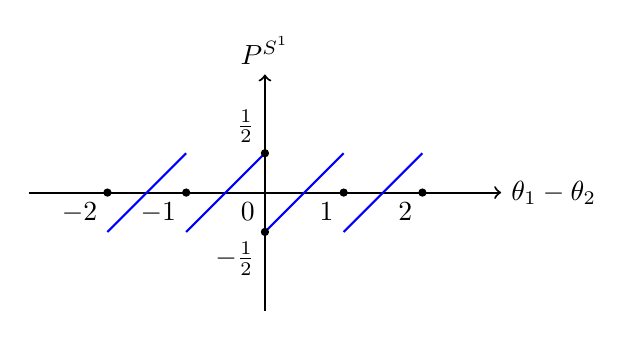
\begin{tikzpicture}
    \draw [->] (-3, 0) -- (3, 0) node [right] {$\theta_1-\theta_2$};
    \draw [->] (0, -1.5) -- (0, 1.5) node [above] {$P^{S^1}$};

    \node [anchor = north east] at (-2, 0) {$-2$};
    \node [anchor = north east] at (-1, 0) {$-1$};
    \node [anchor = north east] at (0, 0) {$0$};
    \node [anchor = north east] at (1, 0) {$1$};
    \node [anchor = north east] at (2, 0) {$2$};
    
    \foreach \x in {-2, -1, 0, 1} {
      \draw [blue] (\x, -0.5) -- (\x + 1, 0.5);
    }
    \node [anchor = south east] at (0, 0.5) {$\frac{1}{2}$};
    \node [anchor = north east] at (0, -0.5) {$-\frac{1}{2}$};
    
    \node [fill, circle, inner sep = 0, minimum size = 3] at (0, 0.5) {};
    \node [fill, circle, inner sep = 0, minimum size = 3] at (0, -0.5) {};
    \node [fill, circle, inner sep = 0, minimum size = 3] at (-2, 0) {};
    \node [fill, circle, inner sep = 0, minimum size = 3] at (-1, 0) {};
    \node [fill, circle, inner sep = 0, minimum size = 3] at (1, 0) {};
    \node [fill, circle, inner sep = 0, minimum size = 3] at (2, 0) {};
\end{tikzpicture}\eea
$P^{S^1}$ is NOT a smooth function on $S^1 \times S^1$ (as expected), but it is \emph{bounded}.
\end{prop}

\subsection*{Correlation map}
Let us denote the formal Weyl algebra
\bea \cW_{2n}= \lb \bR \llb p_i,q^i\rrb ((\hbar)), \ast\rb,\eea
and the formal Weyl subalgebra
\bea \cW_{2n}^+ = \lb \bR \llb p_i,q^i\rrb \llb\hbar\rrb, \ast\rb,\eea
where $\ast$ is the Moyal-Weyl product. We can identify the formal Weyl subalgebra as (formal) functions on $V$ (via deformation quantization):
\bea \cW_{2n}^+ \simeq \lb\widehat{\sO}(V)\llb \hbar\rrb, \ast\rb. \eea
Given $f_0,f_1,\cdots, f_m \in \cW_{2n}$, define
$\cO_{f_0,f_1,\cdots, f_m} \in \sO(\cE)((\hbar))$
by
\bea \cO_{f_0,f_1,\cdots, f_m}\lsb \varphi\rsb\coloneqq \int_{0<\theta_1<\theta_2<\cdots<\theta_m<1} d\theta_1 d\theta_2 \cdots d\theta_m f^{(0)}_{0}\lb \varphi(\theta_0)\rb f^{(1)}_{1}\lb \varphi(\theta_1)\rb \cdots f^{(1)}_{m}\lb \varphi(\theta_m)\rb, \quad \varphi\in \Omega^\blt_{S^1}\otimes V. \eea
Here $f(\varphi(\theta))=f(\bP_i(\theta),\bQ^i(\theta))\in \Omega^\blt_{S^1}$ 
and we decompose it as 
$f(\varphi(\theta))=f^{(0)}(\varphi(\theta))+f^{(1)}(\varphi(\theta))d\theta$.

\begin{rmk}
$f^{(1)}(\varphi)$ is the \textbf{topological descent} of $f^{(0)}(\varphi)$ (in the sense of Witten).
\end{rmk}

Now let's apply the homotopy RG flow, $\exp{(\hbar P^\infty_0)}\lb \cO_{f_0,f_1,\cdots, f_m}\rb$. Since $P^\infty_0$ is bounded, it is convergent and well-defined! This is a \emph{UV finite property}.

As we have discussed, at $L=\infty$, we can view it as defining a function on zero modes on 
\bea\bH &=H^\blt\lb \Omega^\blt_{S^1} \otimes V, d\rb= H^\blt(S^1)\otimes V\\
&= V\oplus V d\theta.\eea
We have $\widehat{\sO}(\bH)=\widehat{\Omega}^{-\blt}_{2n}$ forms on $V$.

\begin{defn}
We define the following correlation map:
\bea \lan \cdots\ran_{free}: \cW_{2n} \otimes \cdots \otimes \cW_{2n} \to \widehat{\Omega}^{-\blt}_{2n}((\hbar))\eea
by $\lan f_0\otimes f_1\otimes \cdots\otimes f_m\ran_{free} \coloneqq \left. \exp{(\hbar P^\infty_0)}\lb \cO_{f_0,f_1,\cdots, f_m}\rb \right|_{\bH}$.
In the path integral perspective, this is 
\bea \lan f_0\otimes f_1\otimes \cdots\otimes f_m\ran_{free}(\alpha)
=\int_{\Im d^\ast \subset \cE} \lsb D\varphi\rsb e^{-S[\varphi+\alpha]/\hbar} \cO_{f_0,f_1,\cdots,f_m}[\varphi+\alpha], \quad \alpha\in \bH= H^\blt(S^1)\otimes V.\eea
$\alpha$ is essentially the background field. It can also be represented as a Feynman diagram as follows.
\begin{figure}[!htpb]\centering 
\tikzset{every picture/.style={line width=0.75pt}} %set default line width to 0.75pt        
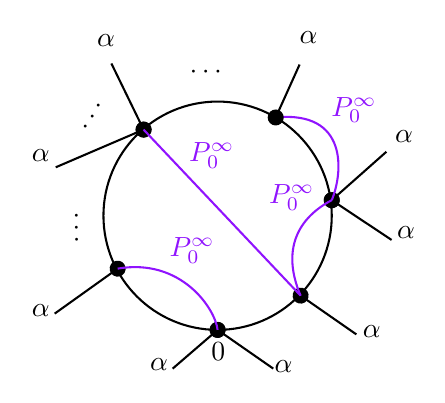
\begin{tikzpicture}[x=0.75pt,y=0.75pt,yscale=-1,xscale=1]
%uncomment if require: \path (0,300); %set diagram left start at 0, and has height of 300

%Shape: Circle [id:dp32266046359972234] 
\draw   (370.33,193.5) .. controls (370.33,163.12) and (394.96,138.5) .. (425.33,138.5) .. controls (455.71,138.5) and (480.33,163.12) .. (480.33,193.5) .. controls (480.33,223.88) and (455.71,248.5) .. (425.33,248.5) .. controls (394.96,248.5) and (370.33,223.88) .. (370.33,193.5) -- cycle ;
%Straight Lines [id:da8359020571133517] 
\draw    (374.17,120.17) -- (389.67,152) ;
\draw [shift={(389.67,152)}, rotate = 64.04] [color={rgb, 255:red, 0; green, 0; blue, 0 }  ][fill={rgb, 255:red, 0; green, 0; blue, 0 }  ][line width=0.75]      (0, 0) circle [x radius= 3.35, y radius= 3.35]   ;
%Straight Lines [id:da7986088148712582] 
\draw    (347.33,170.17) -- (389.67,152) ;
\draw [shift={(389.67,152)}, rotate = 336.77] [color={rgb, 255:red, 0; green, 0; blue, 0 }  ][fill={rgb, 255:red, 0; green, 0; blue, 0 }  ][line width=0.75]      (0, 0) circle [x radius= 3.35, y radius= 3.35]   ;
%Straight Lines [id:da8708432649210969] 
\draw    (346.83,240.67) -- (377.17,219) ;
\draw [shift={(377.17,219)}, rotate = 324.46] [color={rgb, 255:red, 0; green, 0; blue, 0 }  ][fill={rgb, 255:red, 0; green, 0; blue, 0 }  ][line width=0.75]      (0, 0) circle [x radius= 3.35, y radius= 3.35]   ;
%Straight Lines [id:da15766790265263397] 
\draw    (403.67,267.17) -- (425.33,248.5) ;
\draw [shift={(425.33,248.5)}, rotate = 319.25] [color={rgb, 255:red, 0; green, 0; blue, 0 }  ][fill={rgb, 255:red, 0; green, 0; blue, 0 }  ][line width=0.75]      (0, 0) circle [x radius= 3.35, y radius= 3.35]   ;
%Straight Lines [id:da17957602222249913] 
\draw    (452.17,267.17) -- (425.33,248.5) ;
\draw [shift={(425.33,248.5)}, rotate = 214.82] [color={rgb, 255:red, 0; green, 0; blue, 0 }  ][fill={rgb, 255:red, 0; green, 0; blue, 0 }  ][line width=0.75]      (0, 0) circle [x radius= 3.35, y radius= 3.35]   ;
%Straight Lines [id:da3682811688121579] 
\draw    (492.17,250.67) -- (465.33,232) ;
\draw [shift={(465.33,232)}, rotate = 214.82] [color={rgb, 255:red, 0; green, 0; blue, 0 }  ][fill={rgb, 255:red, 0; green, 0; blue, 0 }  ][line width=0.75]      (0, 0) circle [x radius= 3.35, y radius= 3.35]   ;
%Straight Lines [id:da6871435476196512] 
\draw    (509.17,205.17) -- (480.33,186) ;
\draw [shift={(480.33,186)}, rotate = 213.61] [color={rgb, 255:red, 0; green, 0; blue, 0 }  ][fill={rgb, 255:red, 0; green, 0; blue, 0 }  ][line width=0.75]      (0, 0) circle [x radius= 3.35, y radius= 3.35]   ;
%Straight Lines [id:da2213504058401865] 
\draw    (506.67,162.67) -- (480.33,186) ;
\draw [shift={(480.33,186)}, rotate = 138.46] [color={rgb, 255:red, 0; green, 0; blue, 0 }  ][fill={rgb, 255:red, 0; green, 0; blue, 0 }  ][line width=0.75]      (0, 0) circle [x radius= 3.35, y radius= 3.35]   ;
%Curve Lines [id:da8638832915566401] 
\draw [color={rgb, 255:red, 144; green, 19; blue, 254 }  ,draw opacity=1 ]   (377.17,219) .. controls (407.67,213.67) and (424.17,238.17) .. (425.33,248.5) ;
%Curve Lines [id:da033505788594483166] 
\draw [color={rgb, 255:red, 144; green, 19; blue, 254 }  ,draw opacity=1 ]   (480.33,186) .. controls (461.5,196) and (457,212.5) .. (465.33,232) ;
%Curve Lines [id:da045835240771453956] 
\draw [color={rgb, 255:red, 144; green, 19; blue, 254 }  ,draw opacity=1 ]   (453.33,146.17) .. controls (488.33,142.67) and (485.83,172.67) .. (480.33,186) ;
%Straight Lines [id:da3518391071014495] 
\draw    (464.83,120.67) -- (453.33,146.17) ;
\draw [shift={(453.33,146.17)}, rotate = 114.27] [color={rgb, 255:red, 0; green, 0; blue, 0 }  ][fill={rgb, 255:red, 0; green, 0; blue, 0 }  ][line width=0.75]      (0, 0) circle [x radius= 3.35, y radius= 3.35]   ;
%Straight Lines [id:da5327889741402634] 
\draw [color={rgb, 255:red, 144; green, 19; blue, 254 }  ,draw opacity=1 ]   (389.67,152) -- (465.33,232) ;

% Text Node
\draw (400.67,202.4) node [anchor=north west][inner sep=0.75pt]  [color={rgb, 255:red, 144; green, 19; blue, 254 }  ,opacity=1 ]  {$P_{0}^{\infty }$};
% Text Node
\draw (410.17,156.9) node [anchor=north west][inner sep=0.75pt]  [color={rgb, 255:red, 144; green, 19; blue, 254 }  ,opacity=1 ]  {$P_{0}^{\infty }$};
% Text Node
\draw (448.67,176.9) node [anchor=north west][inner sep=0.75pt]  [color={rgb, 255:red, 144; green, 19; blue, 254 }  ,opacity=1 ]  {$P_{0}^{\infty }$};
% Text Node
\draw (478.67,134.9) node [anchor=north west][inner sep=0.75pt]  [color={rgb, 255:red, 144; green, 19; blue, 254 }  ,opacity=1 ]  {$P_{0}^{\infty }$};
% Text Node
\draw (334.33,234.9) node [anchor=north west][inner sep=0.75pt]    {$\alpha $};
% Text Node
\draw (334.33,159.9) node [anchor=north west][inner sep=0.75pt]    {$\alpha $};
% Text Node
\draw (365.83,104.9) node [anchor=north west][inner sep=0.75pt]    {$\alpha $};
% Text Node
\draw (391.33,260.9) node [anchor=north west][inner sep=0.75pt]    {$\alpha $};
% Text Node
\draw (451.33,261.9) node [anchor=north west][inner sep=0.75pt]    {$\alpha $};
% Text Node
\draw (493.83,244.9) node [anchor=north west][inner sep=0.75pt]    {$\alpha $};
% Text Node
\draw (510.33,197.4) node [anchor=north west][inner sep=0.75pt]    {$\alpha $};
% Text Node
\draw (509.33,150.9) node [anchor=north west][inner sep=0.75pt]    {$\alpha $};
% Text Node
\draw (463.33,103.4) node [anchor=north west][inner sep=0.75pt]    {$\alpha $};
% Text Node
\draw (353.34,208.55) node [anchor=north west][inner sep=0.75pt]  [rotate=-269.59]  {$\cdots $};
% Text Node
\draw (410.4,119.77) node [anchor=north west][inner sep=0.75pt]  [rotate=-0.52]  {$\cdots $};
% Text Node
\draw (420.83,253.4) node [anchor=north west][inner sep=0.75pt]    {$0$};
% Text Node
\draw (356.67,151.21) node [anchor=north west][inner sep=0.75pt]  [rotate=-302.24]  {$\cdots $};
\end{tikzpicture}
\end{figure}
\end{defn}

\paragraph{(Cyclic) Hochschild complex reviewed.}
Let $A$ be a unital associative algebra. $\ols{A}=A/(\bC\cdot 1)$. Let $C_{-p}(A)\coloneqq A\otimes \ols{A}^{\otimes p}$ be the cyclic $p$-chains. Define the \textbf{Hochschild differential}
\bea b: C_{-p}(A) \to C_{-p+1}(A), \quad p\geq 1\eea
by $b(a_0\otimes \cdots\otimes a_p)=(-1)^{p} a_p a_0\otimes \cdots\otimes a_{p-1}+\sum_{i=0}^{p-1} (-1)^i a_0\otimes \cdots\otimes a_{i}a_{i+1} \otimes\cdots\otimes a_p$. 
\bea
\tikzset{every picture/.style={line width=0.75pt}} %set default line width to 0.75pt
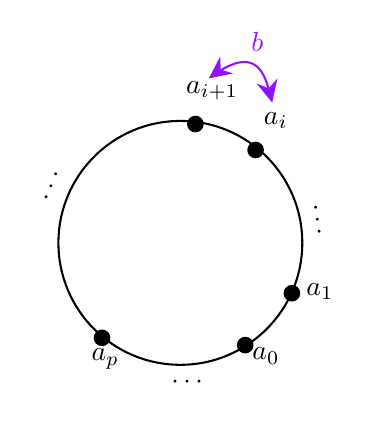
\begin{tikzpicture}[x=0.75pt,y=0.75pt,yscale=-1,xscale=1]
%uncomment if require: \path (0,300); %set diagram left start at 0, and has height of 300

%Shape: Circle [id:dp08860286605746626] 
\draw   (150,161.58) .. controls (150,129.14) and (176.3,102.83) .. (208.75,102.83) .. controls (241.2,102.83) and (267.5,129.14) .. (267.5,161.58) .. controls (267.5,194.03) and (241.2,220.33) .. (208.75,220.33) .. controls (176.3,220.33) and (150,194.03) .. (150,161.58) -- cycle ;
%Shape: Circle [id:dp18094270637610665] 
\draw  [fill={rgb, 255:red, 0; green, 0; blue, 0 }  ,fill opacity=1 ] (212.5,104.33) .. controls (212.5,102.4) and (214.07,100.83) .. (216,100.83) .. controls (217.93,100.83) and (219.5,102.4) .. (219.5,104.33) .. controls (219.5,106.27) and (217.93,107.83) .. (216,107.83) .. controls (214.07,107.83) and (212.5,106.27) .. (212.5,104.33) -- cycle ;
%Shape: Circle [id:dp41020865754033276] 
\draw  [fill={rgb, 255:red, 0; green, 0; blue, 0 }  ,fill opacity=1 ] (241.5,116.83) .. controls (241.5,114.9) and (243.07,113.33) .. (245,113.33) .. controls (246.93,113.33) and (248.5,114.9) .. (248.5,116.83) .. controls (248.5,118.77) and (246.93,120.33) .. (245,120.33) .. controls (243.07,120.33) and (241.5,118.77) .. (241.5,116.83) -- cycle ;
%Shape: Circle [id:dp856537066530171] 
\draw  [fill={rgb, 255:red, 0; green, 0; blue, 0 }  ,fill opacity=1 ] (259,185.83) .. controls (259,183.9) and (260.57,182.33) .. (262.5,182.33) .. controls (264.43,182.33) and (266,183.9) .. (266,185.83) .. controls (266,187.77) and (264.43,189.33) .. (262.5,189.33) .. controls (260.57,189.33) and (259,187.77) .. (259,185.83) -- cycle ;
%Shape: Circle [id:dp6890242736722705] 
\draw  [fill={rgb, 255:red, 0; green, 0; blue, 0 }  ,fill opacity=1 ] (236.5,210.83) .. controls (236.5,208.9) and (238.07,207.33) .. (240,207.33) .. controls (241.93,207.33) and (243.5,208.9) .. (243.5,210.83) .. controls (243.5,212.77) and (241.93,214.33) .. (240,214.33) .. controls (238.07,214.33) and (236.5,212.77) .. (236.5,210.83) -- cycle ;
%Shape: Circle [id:dp026693893451235295] 
\draw  [fill={rgb, 255:red, 0; green, 0; blue, 0 }  ,fill opacity=1 ] (167.5,207.33) .. controls (167.5,205.4) and (169.07,203.83) .. (171,203.83) .. controls (172.93,203.83) and (174.5,205.4) .. (174.5,207.33) .. controls (174.5,209.27) and (172.93,210.83) .. (171,210.83) .. controls (169.07,210.83) and (167.5,209.27) .. (167.5,207.33) -- cycle ;
%Curve Lines [id:da5772031059488538] 
\draw [color={rgb, 255:red, 144; green, 19; blue, 254 }  ,draw opacity=1 ]   (224.93,80.57) .. controls (244.95,66.62) and (249.34,79.1) .. (252.3,91.1) ;
\draw [shift={(253,94)}, rotate = 256.48] [fill={rgb, 255:red, 144; green, 19; blue, 254 }  ,fill opacity=1 ][line width=0.08]  [draw opacity=0] (10.72,-5.15) -- (0,0) -- (10.72,5.15) -- (7.12,0) -- cycle    ;
\draw [shift={(222.5,82.33)}, rotate = 322.94] [fill={rgb, 255:red, 144; green, 19; blue, 254 }  ,fill opacity=1 ][line width=0.08]  [draw opacity=0] (10.72,-5.15) -- (0,0) -- (10.72,5.15) -- (7.12,0) -- cycle    ;

% Text Node
\draw (210,82.23) node [anchor=north west][inner sep=0.75pt]    {$a_{i+1}$};
% Text Node
\draw (247.5,97.23) node [anchor=north west][inner sep=0.75pt]    {$a_{i}$};
% Text Node
\draw (268,179.73) node [anchor=north west][inner sep=0.75pt]    {$a_{1}$};
% Text Node
\draw (242,210.73) node [anchor=north west][inner sep=0.75pt]    {$a_{0}$};
% Text Node
\draw (164.5,211.23) node [anchor=north west][inner sep=0.75pt]    {$a_{p}$};
% Text Node
\draw (241.5,58.4) node [anchor=north west][inner sep=0.75pt]  [color={rgb, 255:red, 144; green, 19; blue, 254 }  ,opacity=1 ]  {$b$};
% Text Node
\draw (146.72,134.32) node  [rotate=-292.57]  {$\cdots $};
% Text Node
\draw (212.22,228.82) node  [rotate=-1.35]  {$\cdots $};
% Text Node
\draw (275.22,150.32) node  [rotate=-261.64]  {$\cdots $};


\end{tikzpicture}
\eea
Then the associativity implies 
\bea b\circ b=0.\eea
Hence, $(C_{-\blt}(A), b)$ is the Hochschild chain complex.

We can also define the \textbf{Connes operator}:
\bea B: C_{-p}(A) \to C_{-p-1}(A)\eea
by $B(a_0\otimes \cdots\otimes a_p)=1\otimes a_0 \otimes\cdots\otimes a_p+\sum_{i=1}^p (-1)^{pi} 1\otimes a_i \otimes\cdots\otimes a_p\otimes a_0 \otimes\cdots\otimes a_{i-1}.$
We have the following relations:
\bea b^2=0, \quad B^2=0, \quad [b,B]=bB+Bb=0.\eea
Let $u$ be a formal variable of $\on{deg}=2$. Then $(b+uB)^2=0$.
This defines a complex
\bea CC^{per}_{-\blt}(A)=\lb C_{-\blt}(A)[u,u^{-1}], b+uB\rb,\eea
called the \textbf{periodic cyclic complex}.

\paragraph{Correlation map.}
It is not hard to see via type reason that
\bea \lan \cdots\ran_{free}: C_{-p}\lb \cW_{2n}\rb \to \widehat{\Omega}^{-p}_{2n}((\hbar)),\eea
i.e. $\lan f_0\otimes f_1\otimes \cdots\otimes f_p\ran_{free}$ is a $p$-form. Recall that $\widehat{\Omega}^{-\blt}_{2n}$ is equipped with a BV operator $\Delta=\cL_{\omega^{-1}}=\cL_\Pi$.

\begin{prop}
\bea \lan b(-)\ran_{free}= \hbar \Delta \lan \cdots\ran_{free},\\
\lan B(-)\ran_{free}= d_{2n} \lan \cdots\ran_{free}.\eea
\end{prop}
Here $d_{2n}: \widehat{\Omega}^{-\blt}_{2n} \to \widehat{\Omega}^{-(\blt+1)}_{2n}$ is the de Rham differential. In other words, the \textbf{correlation map}:
\bea  \lan \cdots\ran_{free}: C_{-\blt}(\cW_{2n}) \to \widehat{\Omega}^{-\blt}_{2n}((\hbar ))\eea
intertwines $b$ with $\hbar\Delta$ and $B$ with $d_{2n}$. We can combine the above two equations and get
\bea \lan\cdots\ran_{free}: CC^{per}_{-\blt}(\cW_{2n})\to 
\widehat{\Omega}^{-\blt}_{2n}((\hbar))[u,u^{-1}], \quad b+uB \mapsto h\Delta+ud_{2n}.\eea

\subsection*{BV integral on zero modes}
We can define a \emph{BV integration} map on the BV algebra $\lb \widehat{\Omega}^{-\blt}_{2n},\Delta\rb$
which is only non-zero on top forms $\widehat{\Omega}^{-2n}_{2n}$ and sends
\bea \beta\in \widehat{\Omega}^{-2n}_{2n} \mapsto \left. \frac{\hbar^n}{n!}\iota^n_\Pi \beta \right|_{p=q=0}.\eea
This is the \textbf{Berezin integral} over the purely fermionic superLagrangian. We can extend this BV integration to an $S^1$-equivariant version by
\bea \int_{BV}: \widehat{\Omega}^{-\blt}_{2n}[u,u^{-1}] \to \bR((\hbar))[u,u^{-1}], \quad \beta\mapsto \left. \lb u^n e^{\hbar\iota_\Pi/u}\beta\rb\right|_{p=q=0}.\eea
Then it has the following property
\bea \int_{BV} \lb \hbar\Delta +ud_{2n}\rb(-)=0\eea

\begin{rmk}
For $\beta\in \widehat{\Omega}^{-\blt}_{2n}$, the equivariant limit
\bea \lim_{u\to\infty} \int_{BV} \beta= \left. \frac{\hbar^n}{n!}\iota_\Pi^n \beta\right|_{p=q=0}\eea
gives back the Berezin integral.
\end{rmk}

Combining the above maps, we define
\bea \Tr \coloneqq \int_{BV}  \circ \lan \cdots\ran_{free}: CC^{per}_{-\blt}(\cW_{2n})\to \bR((\hbar))[u,u^{-1}]\eea
which satisfies the following equation:
\bea\Tr\lb (b+uB)(-)\rb=0.\eea
Therefore $\Tr$ descends to \emph{periodic cyclic homology}. This is essentially the \textbf{Feigin-Felder-Shoikhet} formula.

\paragraph{A graded version.}
We can generalize slightly by considering a graded vector space $V$ with a $\on{deg}=0$ symplectic pairing $\omega$. We still have the canonical quantization $\lb \widehat{\sO}(V)\llb \hbar\rrb,\ast\rb$ and similarly can define the BV algebra of forms $\lb \widehat{\Omega}^{-\blt}_{V},\Delta=\cL_{\omega^{-1}}\rb$.
The same trace map gives 
\bea \lan \cdots\ran_{free}: C_{-\blt}\lb \widehat{\sO}(V)\llb\hbar\rrb\rb\to 
\widehat{\Omega}^{-\blt}_{V}((\hbar)), \quad b\mapsto \hbar\Delta.\eea
Given $\gamma\in \widehat{\sO}(V)\llb\hbar\rrb$, $\on{deg}(\gamma)=1$, it defines an action functional:
\bea I_\gamma= \int_{S^1}\gamma(\varphi) \quad \forall \varphi\in \Omega^\blt(S^1)\otimes V.\eea
Let's treat $I_\gamma$ as an interaction and consider
\bea \underbrace{\hf \int_{S^1} \lan \varphi,d\varphi\ran}_{\text{free part}}
+\underbrace{\int_{S^1} \gamma(\varphi)}_{I_\gamma}.\eea
Then we run the HRG flow to get
\bea e^{\frac{1}{\hbar}I_\gamma[\infty]}\coloneqq \exp{(\hbar P^\infty_0)} e^{\frac{1}{\hbar}I_\gamma}\eea
which is well-defined since $P^\infty_0$ is bounded.

Let's now analyze the QME. By construction,
\bea e^{\frac{1}{\hbar}I_\gamma[\infty]}= \lan 1\otimes e^{\gamma/\hbar}\ran_{free}.\eea
Assume $\gamma\ast \gamma=\hf \lsb \gamma,\gamma\rsb_\ast=0$. Then 
\bea \hbar\Delta e^{\frac{1}{\hbar}I_\gamma[\infty]}= \lan b\lb 1\otimes e^{\gamma/\hbar}\rb \ran_{free}=0.\eea

\begin{prop}[Grady-Li-L]
If $\lsb \gamma,\gamma\rsb_\ast=0$, then the local interaction $I_\gamma= \int_{S^1} \gamma(\varphi)$ defines a family of solutions of effective QME $I_\gamma[L]$ at scale $L>0$ by
\bea e^{\frac{1}{\hbar}I_\gamma[L]}\coloneqq \lim_{\vep\to\infty} \exp{(\hbar p^L_\vep)} e^{\frac{1}{\hbar}I_\gamma}.\eea
\end{prop}














































 